\newpage
\section{Test of the Reverb Effect}
In this part, tests for the reverb effect that show wether it fulfills the requirement are presented. 


\subsection{Test of requirement \autoref{req:reverb1}}
According to \autoref{req:reverb1}, a test was made to ensure that the \gls{reverb} have at least 1000 echo. The test is done by sending a single known sinus impulse intro the \gls{reverb} effect, and afterwards the echo should haven been counted, but the scope have a limitation of 16k samples on each measurements samples, and the plotted version in this subsection is not really easy to count on. Instead the measurement will be compared to the same simulation test for the MATLAB coded \gls{reverb}. The MATLAB plot and the implemented test plot will be situated side by side, than it is easy to compare. This is done with five different frequency. 

\paragraph{impulse response of \SI{20}{\hertz}}

\begin{figure}[htbp!]
    \centering
        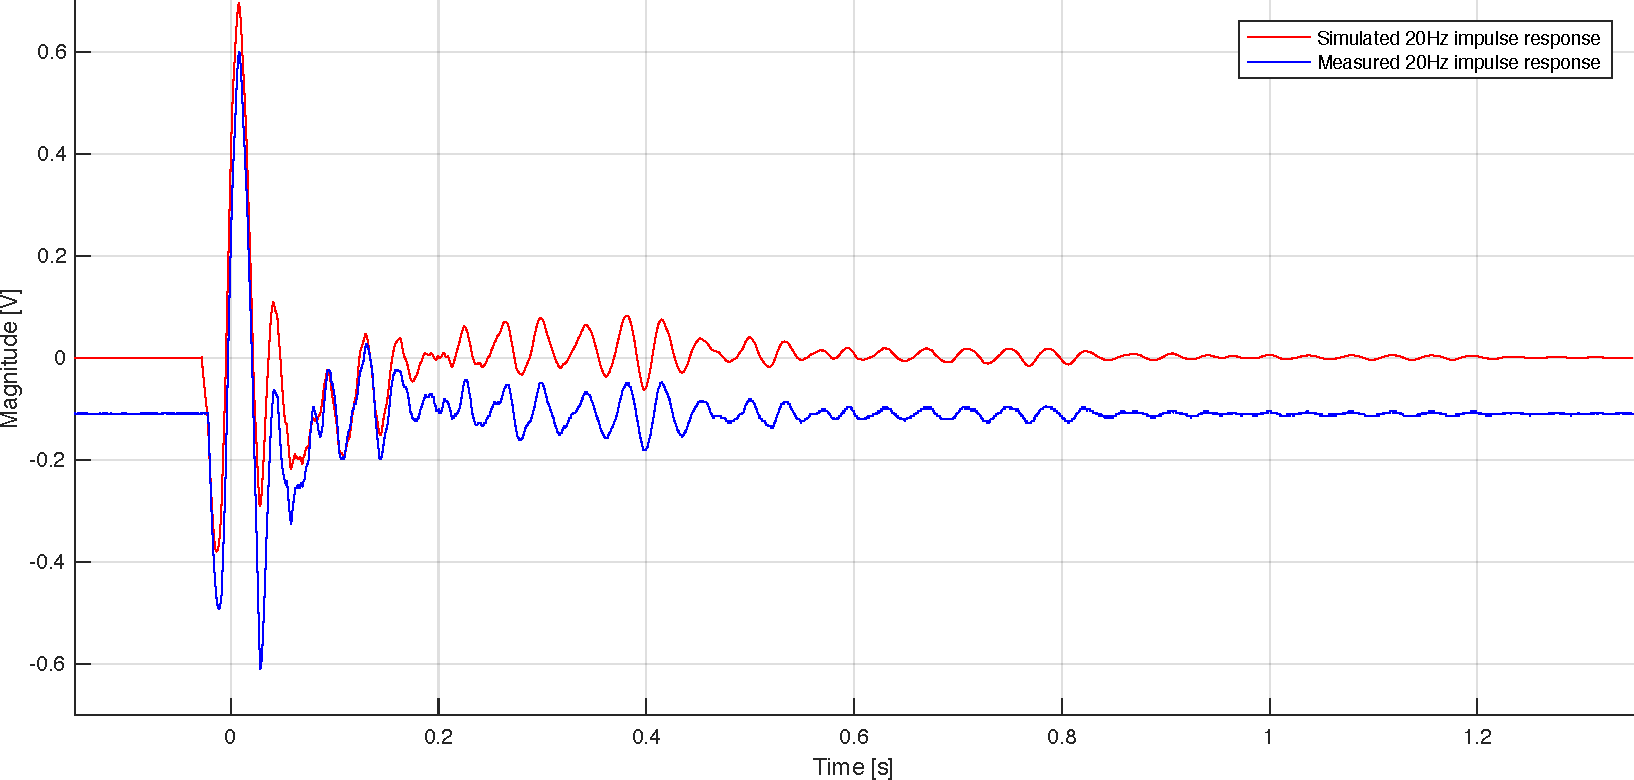
\includegraphics[width=\textwidth]{20Hz_impulse_response.pdf}
        \caption{Plot of the measured and simulated \gls{reverb} impulse response at \SI{20}{\hertz}.}
        \label{fig:tests:reverb:20Hz}
  \end{figure}
  
\paragraph{impulse response of \SI{50}{\hertz}}

\begin{figure}[htbp!]
    \centering
        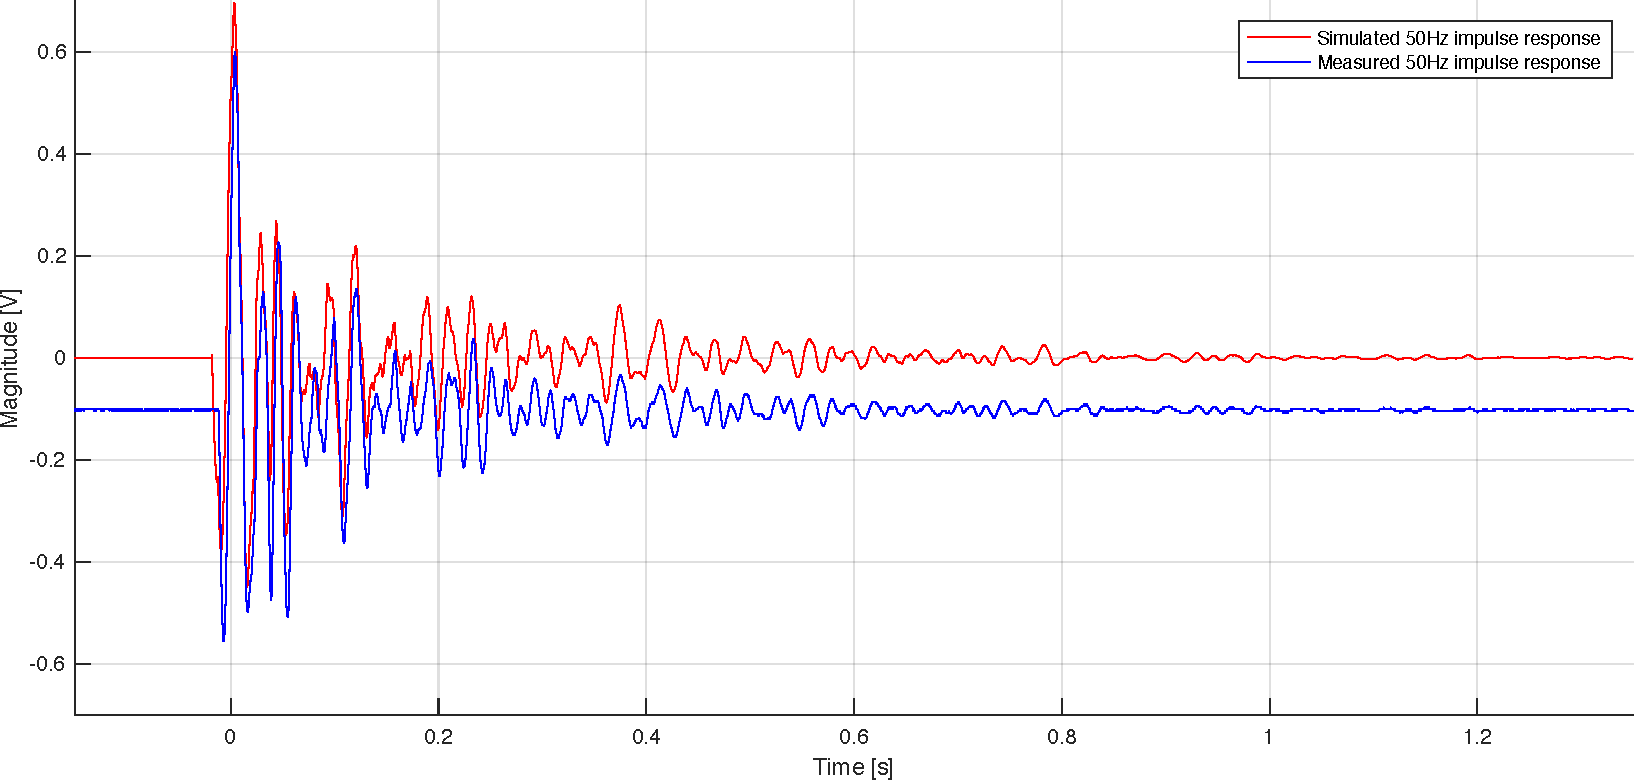
\includegraphics[width=\textwidth]{50Hz_impulse_response.pdf}
        \caption{Plot of the measured and simulated \gls{reverb} impulse response at \SI{50}{\hertz}.}
        \label{fig:tests:reverb:50Hz}
  \end{figure}

\paragraph{impulse response of \SI{200}{\hertz}}

\begin{figure}[htbp!]
    \centering
        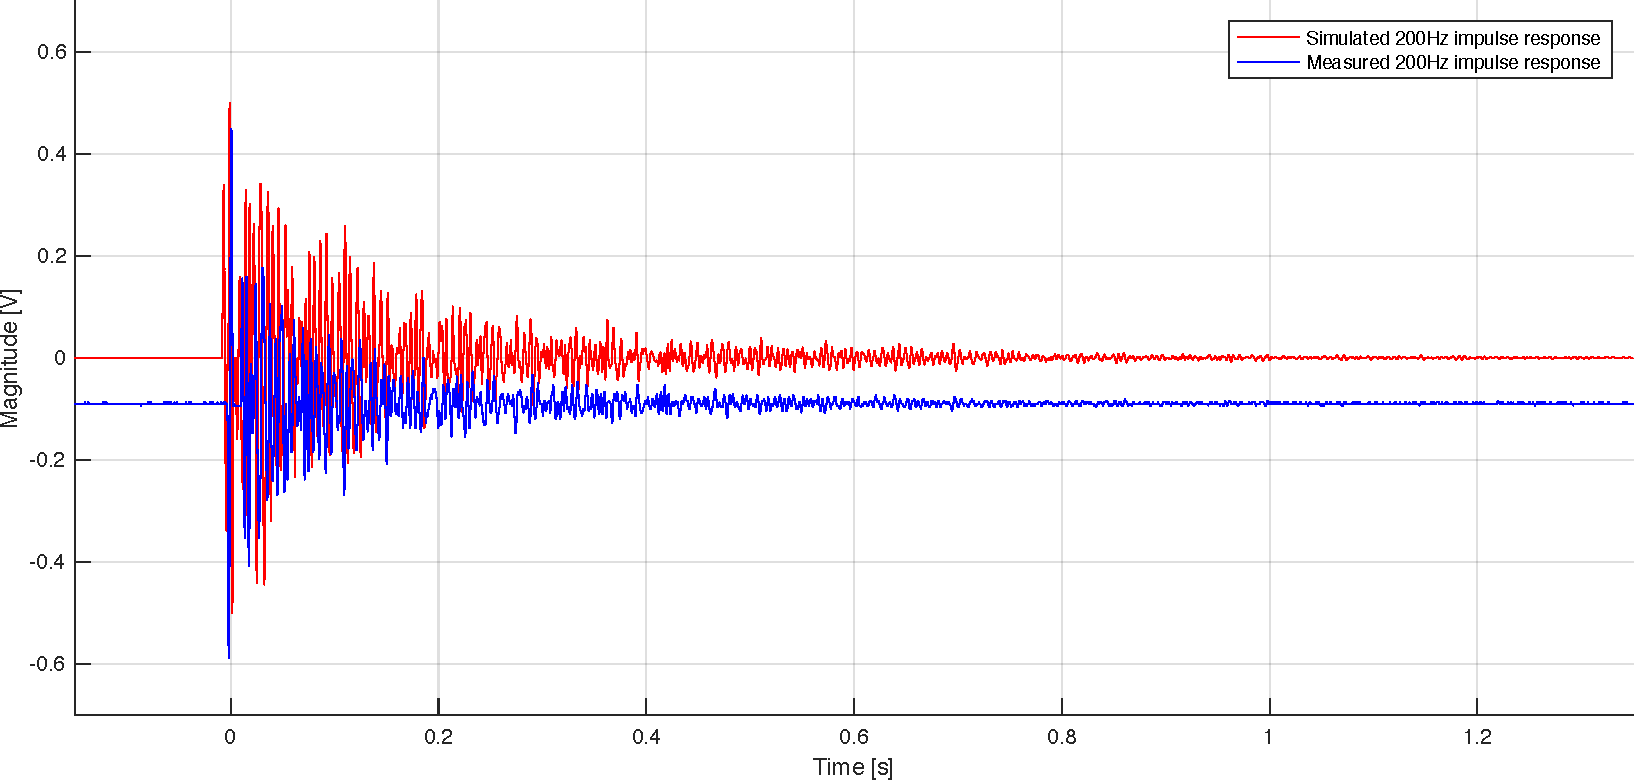
\includegraphics[width=\textwidth]{200Hz_impulse_response.pdf}
        \caption{Plot of the measured and simulated \gls{reverb} impulse response at \SI{200}{\hertz}.}
        \label{fig:tests:reverb:200Hz}
  \end{figure}

\paragraph{impulse response of \SI{1}{\kilo\hertz}}

\begin{figure}[htbp!]
    \centering
        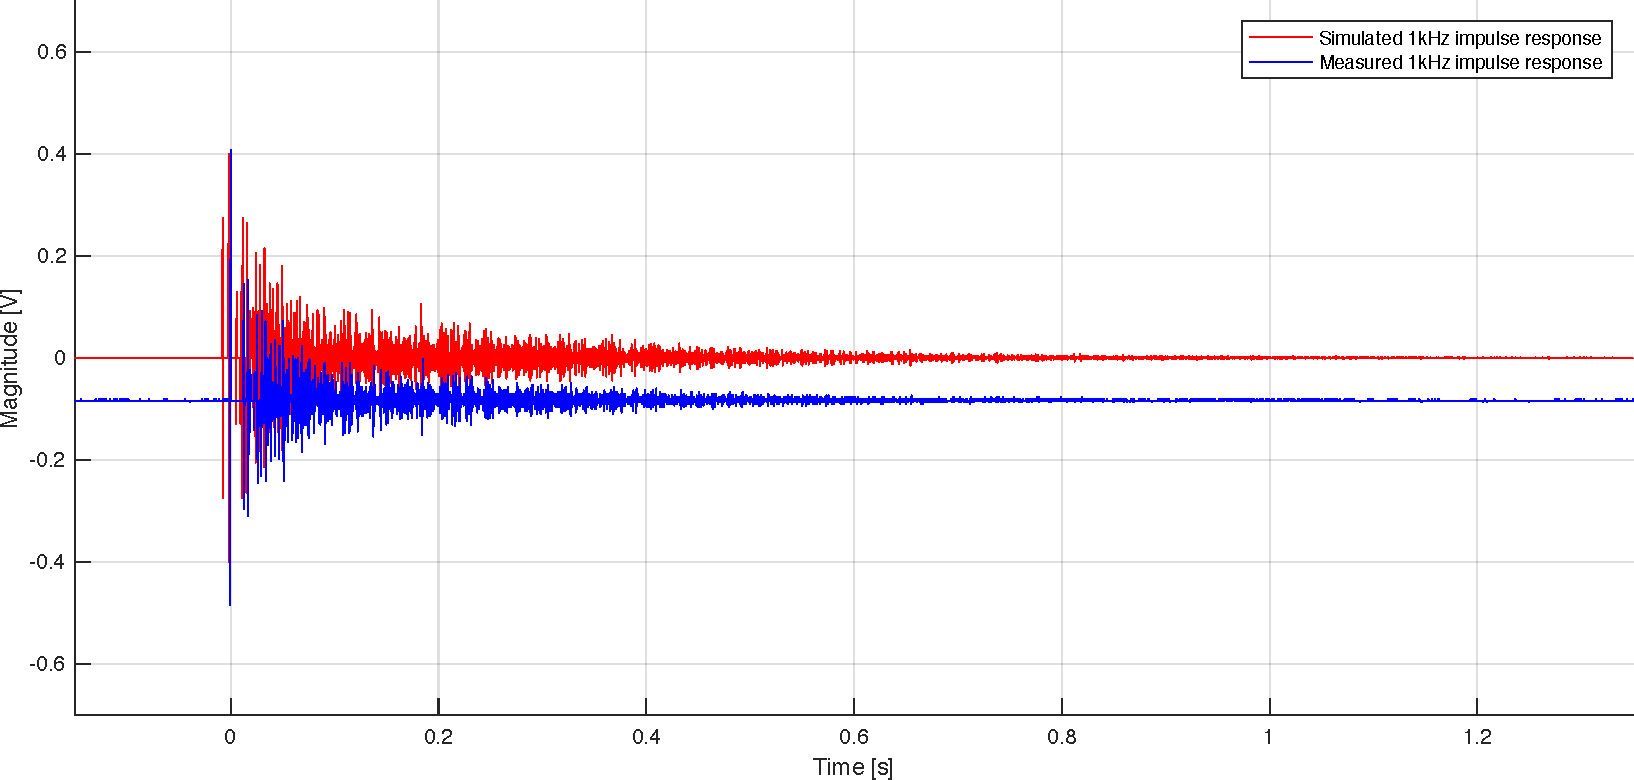
\includegraphics[width=\textwidth]{1kHz_impulse_response.pdf}
        \caption{Plot of the measured and simulated \gls{reverb} impulse response at \SI{1}{\kilo\hertz}.}
        \label{fig:tests:reverb:1kHz}
  \end{figure}
  
  
 \paragraph{impulse response of \SI{5}{\kilo\hertz}}

\begin{figure}[htbp!]
    \centering
        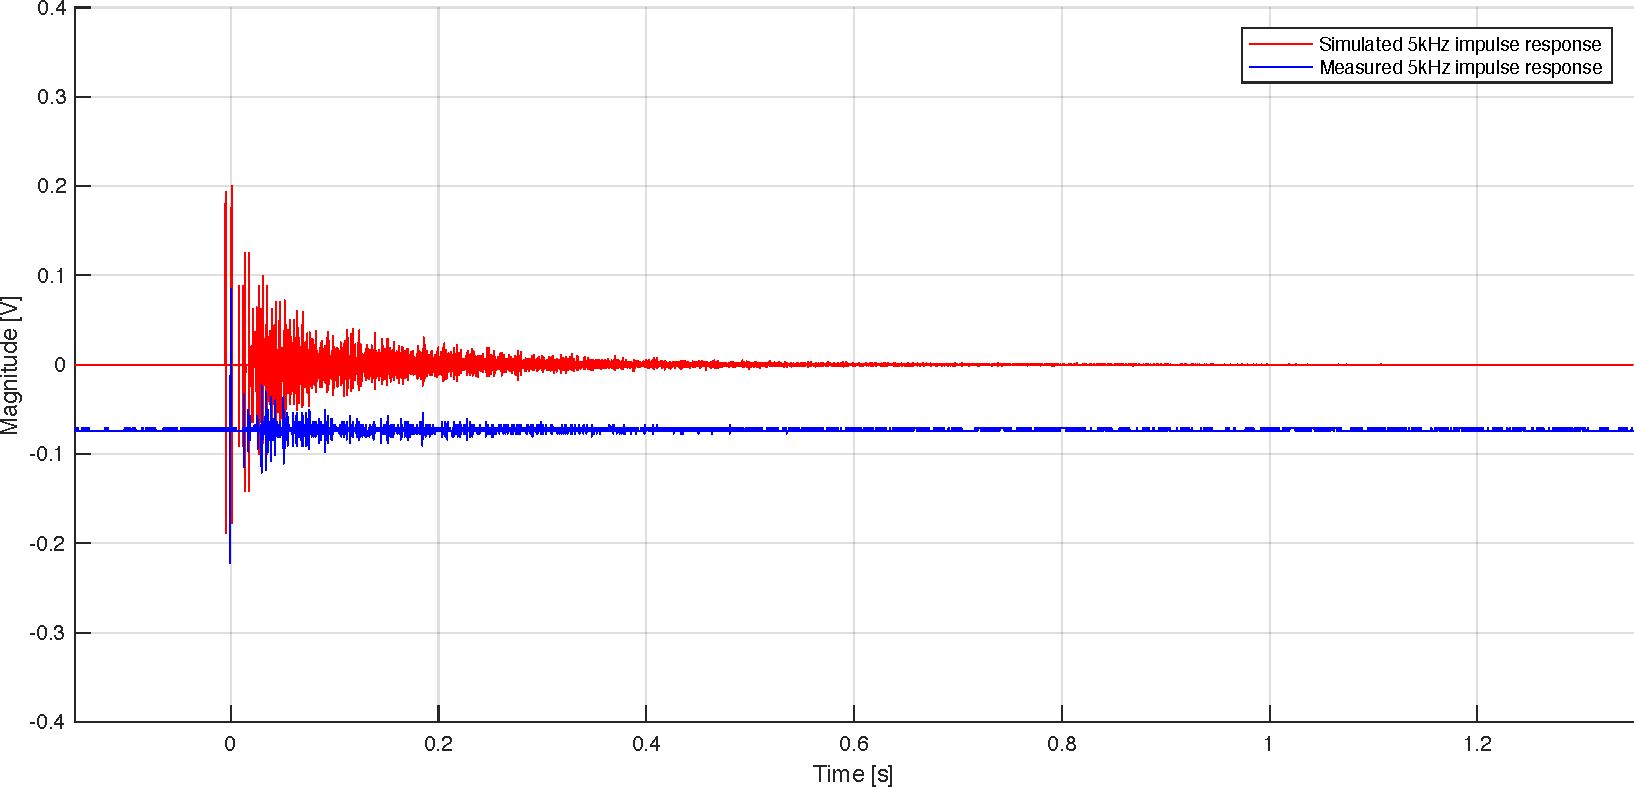
\includegraphics[width=\textwidth]{5kHz_impulse_response.pdf}
        \caption{Plot of the measured and simulated \gls{reverb} impulse response at \SI{5}{\kilo\hertz}.}
        \label{fig:tests:reverb:5kHz}
  \end{figure}
  
  
\subsection{Test of requirement \autoref{req:reverb2}}

\subsection{Test of requirement \autoref{req:reverb3}}

